\documentclass[11pt]{article}
\usepackage[utf8]{inputenc}
\usepackage{amsmath, amsfonts, amssymb}
\usepackage{graphicx}
\usepackage{geometry}
\usepackage{booktabs}
\usepackage{hyperref}
% normalem is required: plain \usepackage{ulem} redefines \emph to underline instead of
% italicise, which silently underlines every \emph in the document -- and, because
% algorithm2e's \ArgSty is \emph, every function argument in every algorithm as well.
% \uline still underlines where it is asked for explicitly.
\usepackage[normalem]{ulem}
\usepackage{microtype}
\usepackage{xcolor}
\usepackage[most]{tcolorbox}
\usepackage{placeins}

% Every algorithm below is placed with [H], i.e. not as a float: it stays exactly where
% it is written, and the surrounding \color reaches it -- a floated algorithm would be
% shipped out after the colour group had closed and would come out black.
\usepackage[ruled,vlined,linesnumbered]{algorithm2e}
% Every name below is the identifier the code actually uses, so the pseudocode and
% src/homework3/ can be read against each other line for line.
\SetKwProg{Fn}{Function}{:}{}
\SetKwFunction{BoxSystem}{BoxSystem}
\SetKwFunction{Splu}{splu}
\SetKwFunction{BoxSolve}{system.solve}
\SetKwFunction{Midpoints}{\_midpoints}
\SetKwFunction{CellSlab}{slab.cell\_flux}
\SetKwFunction{CellSph}{sphere.cell\_flux}
\SetKwFunction{SweepBack}{sweep\_backward}
\SetKwFunction{SweepFwd}{sweep\_forward}
\SetKwFunction{SweepAll}{sweep\_all\_angles}
\SetKwFunction{StartDir}{\_starting\_direction}
\SetKwFunction{RunSn}{run\_sn\_for\_source}
\SetKwFunction{KEig}{k\_eigenvalue}
\SetKwFunction{CritSize}{critical\_size}
\SetKwFunction{Brentq}{brentq}

% Third argument passes extra tcolorbox keys; existing two-argument uses are unaffected.
% It is how the algorithm boxes set coltext: a plain \color inside a breakable box is lost
% at the page break, since each part re-enters with the ambient colour.
\DeclareTColorBox{notebox}{ O{Note} O{blue} O{} }{
  breakable,
  colback=#2!5!white,
  colframe=#2!75!black,
  fonttitle=\bfseries,
  title={#1},
  #3
}

\geometry{margin=1in}

\title{Homework Assignment 3: Critical Systems by Diffusion, $P_N$ and $S_N$}
\author{Tal Ramot}
\date{\today}

\begin{document}

\maketitle

\FloatBarrier
\section*{Question 1: Critical radius of a reflected sphere}
\subsection*{The diffusion equation}



\subsection*{The two regions}

Every radius here is measured in mean free paths of the medium it sits in:
\begin{equation}
    a = \Sigma_{t,C}\,R_C, \qquad\qquad b = \Sigma_{t,R}\,R_R = a + d
    \label{eq:optradii}
\end{equation}
the dimensionless core radius and the dimensionless outer radius of the reflector, whose width is the given $d$.

In both regions the substitution $u(r) = r\phi(r)$, which uses $\frac{1}{r^2}\frac{d}{dr}\left(r^2\frac{d\phi}{dr}\right) = \frac{1}{r}\frac{d^2u}{dr^2}$, turns the spherical diffusion equation into a plane one:
\begin{equation}
    \frac{d^2 u}{dr^2} - \frac{(1-c)\Sigma_t^2}{D_0}\,u = 0
\end{equation}
from which the scalar flux is calculated to be (see slide 2 in Heizler's relevant presentation):
\begin{equation}
    \phi_C(r) = A\,\frac{\sin\!\left(k_0(c_C)\,\Sigma_{t,C}\,r\right)}{\Sigma_{t,C}\,r},
    \qquad\qquad
    \phi_R(r) = F\,\frac{\sinh\!\left(\left[b + z_0(c_R) - \Sigma_{t,R}\,r\right] / \nu_0(c_R)\right)}{\Sigma_{t,R}\,r}
\end{equation}
\paragraph{Derivation.} The core has $c_C > 1$, so the coefficient is negative and the solution oscillates. Finiteness at the origin selects the sine. The reflector has $c_R \le 1$ and decays, vanishing $z_0(c_R)$ mean free paths past $b$. The relaxation rate is $k_0(c_C) = \sqrt{(c_C-1)/D_0(c_C)}$ per mean free path in the core and $1/\nu_0(c_R)=\sqrt{(1-c_R)/D_0(c_R)}$ in the reflector. But remember! $k_0$ and $\nu_0$ are Case's discrete eigenvalues on its two branches (for c smaller or greater than 1), following the identities: $c\,\text{arctan}(k_0) = k_0$ for $c>1$ and $\text{artanh}(1/\nu_0)/(1/\nu_0) = 1/c$ otherwise.

\subsection*{Matching, and the three criticality equations}
The interface at $r = R_C$ carries a flux relation $\phi_R = \rho_{2/1}\,\phi_C$ and a current relation with jump factor $j_{2/1}$. The two continuous approximations set $\rho_{2/1} = j_{2/1} = 1$ and impose both on $\phi$ itself. The discontinuous one takes its two ratios from the plane two-region problem, where $u = r\phi$ plays the part of the plane flux, and so imposes them on $u$. Each set gives one transcendental equation for $a$, and the three cases (a), (b), (c) are the two equations filled with the parameters of Table~1.

\paragraph{(a) and (b): $\phi$ and the net current continuous.} The conditions are
\begin{gather}
    \phi_R(R_C) = \phi_C(R_C) \\
    -\frac{D_R}{\Sigma_R}\left(\frac{d\phi_R(r)}{dr}\right)_{r=R_C} = -\frac{D_C}{\Sigma_C}\left(\frac{d\phi_C(r)}{dr}\right)_{r=R_C}
\end{gather}
In optical variables that current is dimensionless on both sides, $D\,d/dr = D_0\,d/d(\Sigma_t r)$, so $D_R=D_{0,R}$ and $D_C=D_{0,C}$ below are the dimensionless $D_0$ of Table~1. Under substitution of the scalar fluxes the two conditions turn to:
\begin{gather}
    \frac{F}{b-d}\sinh\!\left(\frac{d + z_0(c_R)}{\nu_0(c_R)}\right) = \frac{A}{a}\sin\!\left(k_0(c_C)a\right) \\
    D_R F\left[\frac{\cosh\!\left(\frac{d + z_0(c_R)}{\nu_0(c_R)}\right)}{\nu_0(c_R)\,(b-d)} + \frac{\sinh\!\left(\frac{d + z_0(c_R)}{\nu_0(c_R)}\right)}{(b-d)^2}\right]
    = D_C A\left[\frac{\sin\!\left(k_0(c_C)a\right)}{a^2} - \frac{k_0(c_C)\cos\!\left(k_0(c_C)a\right)}{a}\right]
\end{gather}
divide the two and get:
\begin{equation}
    \boxed{\;\cot\!(k_0a) = \frac{1}{k_0a} - \frac{D_R}{D_C k_0}\left[\frac{1}{\nu_0}\coth\!\left(\frac{d + z_0(c_R)}{\nu_0(c_R)}\right) + \frac{1}{b-d}\right]\;}
    \label{eq:reflcrit}
\end{equation}

\paragraph{(c): the fixed jump conditions.} The \textit{fixed} jump conditions for the curvilinear coordinates under the spherical symmetry relation $\phi \to r\phi$ and Zimmerman's $\rho_{2/1} = \mu_0(c_C)/\mu_0(c_R)$, $j_{2/1} = 1$ are:
\begin{gather}
    \mu_0(c_R)\left[r \phi_R(r)\right]_{r=R_C} = \mu_0(c_C) \left[r\phi_C(r)\right]_{r=R_C} \\
    -\frac{D_R}{\Sigma_R}\left(\frac{d[r\phi_R(r)]}{dr}\right)_{r=R_C} = -\frac{D_C}{\Sigma_C}\left(\frac{d[r\phi_C(r)]}{dr}\right)_{r=R_C}
\end{gather}
which under substitution of the scalar fluxes turn to:
\begin{gather}
    \mu_0(c_R)\frac{F}{\Sigma_{R}}\sinh\!\left(\frac{d + z_0(c_R)}{\nu_0(c_R)}\right) = \mu_0(c_C) \frac{A}{\Sigma_{C}}\sin\!\left(k_0(c_C)a\right) \\
    -\frac{D_R F}{\Sigma_R\nu_0(c_R)}\cosh\!\left(\frac{d + z_0(c_R)}{\nu_0(c_R)}\right) = \frac{j_{2/1} D_C A\,k_0(c_C)}{\Sigma_C} \cos\!\left(k_0(c_C)a\right)
\end{gather} 
divide the two and get:
\begin{equation}
    \boxed{\;\cot\!(k_0a) = -\frac{\mu_0(c_C)}{\mu_0(c_R)}\frac{D_R/\nu_0}{D_C k_0}\coth\!\left(\frac{d + z_0(c_R)}{\nu_0(c_R)}\right)\;}
    \label{eq:reflfixed}
\end{equation}

writing $k_0 = k_0(c_C)$ and $\nu_0 = \nu_0(c_R)$. Notice that $d$ is defined here such that $b - d = \Sigma_{R}R_C$. The code keeps the two conversions apart. The reflector enters through nothing but the optical combination $\left(d + z_0(c_R)\right)/\nu_0(c_R)$, its thickness in its own diffusion lengths. Both equations run from $+\infty$ at $a \to 0$ to $-\infty$ at $a = \pi/k_0$, the unreflected limit, so the fundamental root is always bracketed by $(0,\pi/k_0)$ and \texttt{brentq} finds it in one call.

So the three cases are
\begin{equation*}
    \text{(a)}\;\;\text{with}\;D_0 = \tfrac13,\;z_0 = \tfrac23
    \qquad
    \text{(b)}\;\;\text{with the asymptotic}\;D_0,\,z_0
    \qquad
    \text{(c)}\;\;\text{with the asymptotic}\;D_0,\,z_0
\end{equation*}

The three approximations differ only in what they put into $D_0$ and $z_0$:

\begin{table}[htbp]
\centering
\begin{tabular}{lccc}
\toprule
 & (a) continuous classic & (b) continuous asymptotic & (c) discontinuous asymptotic \\
\midrule
$D_0(c)$ & $1/3$ & $|1-c|\,\nu_0^2$ & $|1-c|\,\nu_0^2$ \\
$z_0(c)$ & $2/3$ & $0.710446\,[1+q(1-c)^2]/c$ & $0.710446\,[1+q(1-c)^2]/c$ \\
$\rho_{2/1} = \phi_R/\phi_C$ & $1$ & $1$ & $\mu_0(c_C)/\mu_0(c_R)$ \\
\bottomrule
\end{tabular}
\caption{The three approximations differ only in what   they put into $D_0$ and $z_0$. The discontinuous one also takes the flux ratio from Zimmerman.}
\end{table}

\paragraph{Zimmerman's $\mu_0$.} The discontinuity comes from Zimmerman, who writes the partial currents of the asymptotic mode as $j_\pm = \tfrac12 \mu_0 \phi_0 \pm \tfrac12 \phi_1$, so that $\mu_0\phi_0 = J_+ + J_-$ is the total traffic across a surface and
\begin{equation}
    \mu_0(c) = \frac{\int_0^1 \mu \psi_{asym} (\mu)d\mu}{\frac{1}{2}\int_{-1}^{1}\psi_{asym}(\mu)d\mu} = \frac{c\,\nu_0^2}{2}\ln\!\left(\frac{\nu_0^2}{\nu_0^2-1}\right)
\end{equation}
where
\begin{equation}
    \qquad
    \nu_0 = \nu_0(c)\;\;\text{for}\;\;c<1,
    \qquad
    |\nu_0| = 1/k_0(c)\;\;\text{for}\;\;c>1
    \label{eq:mu0}
\end{equation}
the second branch being the analytic continuation through $\nu_0 = i/k_0$, which is real and equal to $\tfrac{c}{2k_0^2}\ln(1+k_0^2)$. It returns the two textbook limits $\mu_0 = 1/2$ for an isotropic flux and $\mu_0 = 1$ for a one-way beam.

\begin{table}[htbp]
\centering
\begin{tabular}{lccccccc}
\toprule
material & $c$ & mfp (\Sigma_t^{-1}) [cm] & $k_0$ or $1/\nu_0$ & $D_0$ & $D$ [cm] & $\mu_0$ & $z_0$ \\
\midrule
Pu-239 & 1.5000 & 3.064  & 1.45110 & 0.23745 & 0.7275 & 0.40363 & 0.47127 \\
U-235  & 1.3000 & 3.064  & 1.05708 & 0.26847 & 0.8225 & 0.43639 & 0.54552 \\
H$_2$O & 0.9000 & 3.064  & 0.52543 & 0.36222 & 1.1097 & 0.52660 & 0.78923 \\
Fe     & 0.9980 & 4.300  & 0.07740 & 0.33387 & 1.4356 & 0.50050 & 0.71187 \\
Na     & 1.0000 & 11.578 & 0.00000 & 0.33333 & 3.8595 & 0.50000 & 0.71045 \\
\bottomrule
\end{tabular}
\caption{Asymptotic parameters of the five materials according to their cross-section values from Assignment 1.}
\end{table}

\FloatBarrier
\subsection*{Results}

The bare spheres of Assignment 1 Question 5, which every reflected radius below is measured against:

\begin{table}[htbp]
\centering
\begin{tabular}{ccccc}
\toprule
core & classic $R_c$ [cm] & asympt.\ $R_c$ [cm] & classic $M_c$ [kg] & asympt.\ $M_c$ [kg] \\
\midrule
Pu-239 & 5.8163 & 5.1890 & 12.940 & 9.188 \\
U-235  & 8.1031 & 7.4339 & 42.345 & 32.696 \\
\bottomrule
\end{tabular}
\caption{Bare reference. Theory (a) is compared with the classical column, (b) and (c) with the asymptotic one.}
\end{table}

\begin{table}[htbp]
\centering
\begin{tabular}{cccccccc}
\toprule
reflector & $d$ [mfp] & $R_c^{(a)}$ & $R_c^{(b)}$ & $R_c^{(c)}$ & $M_c^{(a)}$ & $M_c^{(b)}$ & $M_c^{(c)}$ \\
\midrule
Water  & 1  & 5.3159 & 4.9484 & 4.4195 & 9.879  & 7.968  & 5.677 \\
Water  & 2  & 5.0855 & 4.7987 & 4.2459 & 8.649  & 7.267  & 5.034 \\
Water  & 3  & 5.0153 & 4.7499 & 4.1906 & 8.296  & 7.048  & 4.840 \\
Water  & 10 & 4.9814 & 4.7244 & 4.1620 & 8.129  & 6.935  & 4.741 \\
\midrule
Iron   & 1  & 5.4212 & 4.9575 & 4.2252 & 10.478 & 8.013  & 4.961 \\
Iron   & 2  & 5.1056 & 4.7364 & 3.9170 & 8.753  & 6.988  & 3.952 \\
Iron   & 3  & 4.9506 & 4.6237 & 3.7661 & 7.979  & 6.501  & 3.513 \\
Iron   & 10 & 4.6790 & 4.4188 & 3.5037 & 6.737  & 5.674  & 2.829 \\
\midrule
Sodium & 1  & 6.4397 & 5.7159 & 4.2207 & 17.562 & 12.281 & 4.945 \\
Sodium & 2  & 6.3134 & 5.6405 & 3.9087 & 16.549 & 11.801 & 3.927 \\
Sodium & 3  & 6.2505 & 5.6022 & 3.7544 & 16.059 & 11.563 & 3.480 \\
Sodium & 10 & 6.1315 & 5.5286 & 3.4701 & 15.159 & 11.113 & 2.748  \\
\bottomrule
\end{tabular}
\caption{Pu-239 core, critical radius in cm and critical mass in kg, under (a) continuous classic, (b) continuous asymptotic and (c) discontinuous asymptotic diffusion.}
\end{table}

\begin{table}[htbp]
\centering
\begin{tabular}{cccccccc}
\toprule
reflector & $d$ [mfp] & $R_c^{(a)}$ & $R_c^{(b)}$ & $R_c^{(c)}$ & $M_c^{(a)}$ & $M_c^{(b)}$ & $M_c^{(c)}$ \\
\midrule
Water  & 1  & 7.2501 & 6.9113 & 6.4284 & 30.330 & 26.273 & 21.143 \\
Water  & 2  & 6.9185 & 6.6731 & 6.1577 & 26.355 & 23.649 & 18.582 \\
Water  & 3  & 6.8146 & 6.5937 & 6.0691 & 25.186 & 22.816 & 17.791 \\
Water  & 10 & 6.7638 & 6.5520 & 6.0228 & 24.627 & 22.385 & 17.387 \\
\midrule
Iron   & 1  & 7.2811 & 6.8392 & 6.1246 & 30.720 & 25.460 & 18.284 \\
Iron   & 2  & 6.8002 & 6.4625 & 5.6147 & 25.027 & 21.480 & 14.087 \\
Iron   & 3  & 6.5545 & 6.2644 & 5.3543 & 22.411 & 19.565 & 12.217 \\
Iron   & 10 & 6.1125 & 5.8970 & 4.8895 & 18.176 & 16.320 & 9.303 \\
\midrule
Sodium & 1  & 8.4264 & 7.7951 & 6.1175 & 47.618 & 37.697 & 18.220 \\
Sodium & 2  & 8.2322 & 7.6564 & 5.6006 & 44.401 & 35.721 & 13.981 \\
Sodium & 3  & 8.1328 & 7.5844 & 5.3339 & 42.811 & 34.722 & 12.077 \\
Sodium & 10 & 7.9401 & 7.4425 & 4.8292 & 39.840 & 32.809 & 8.963  \\
\bottomrule
\end{tabular}
\caption{U-235 core, same columns.}
\end{table}

\begin{figure}[htbp]
\centering
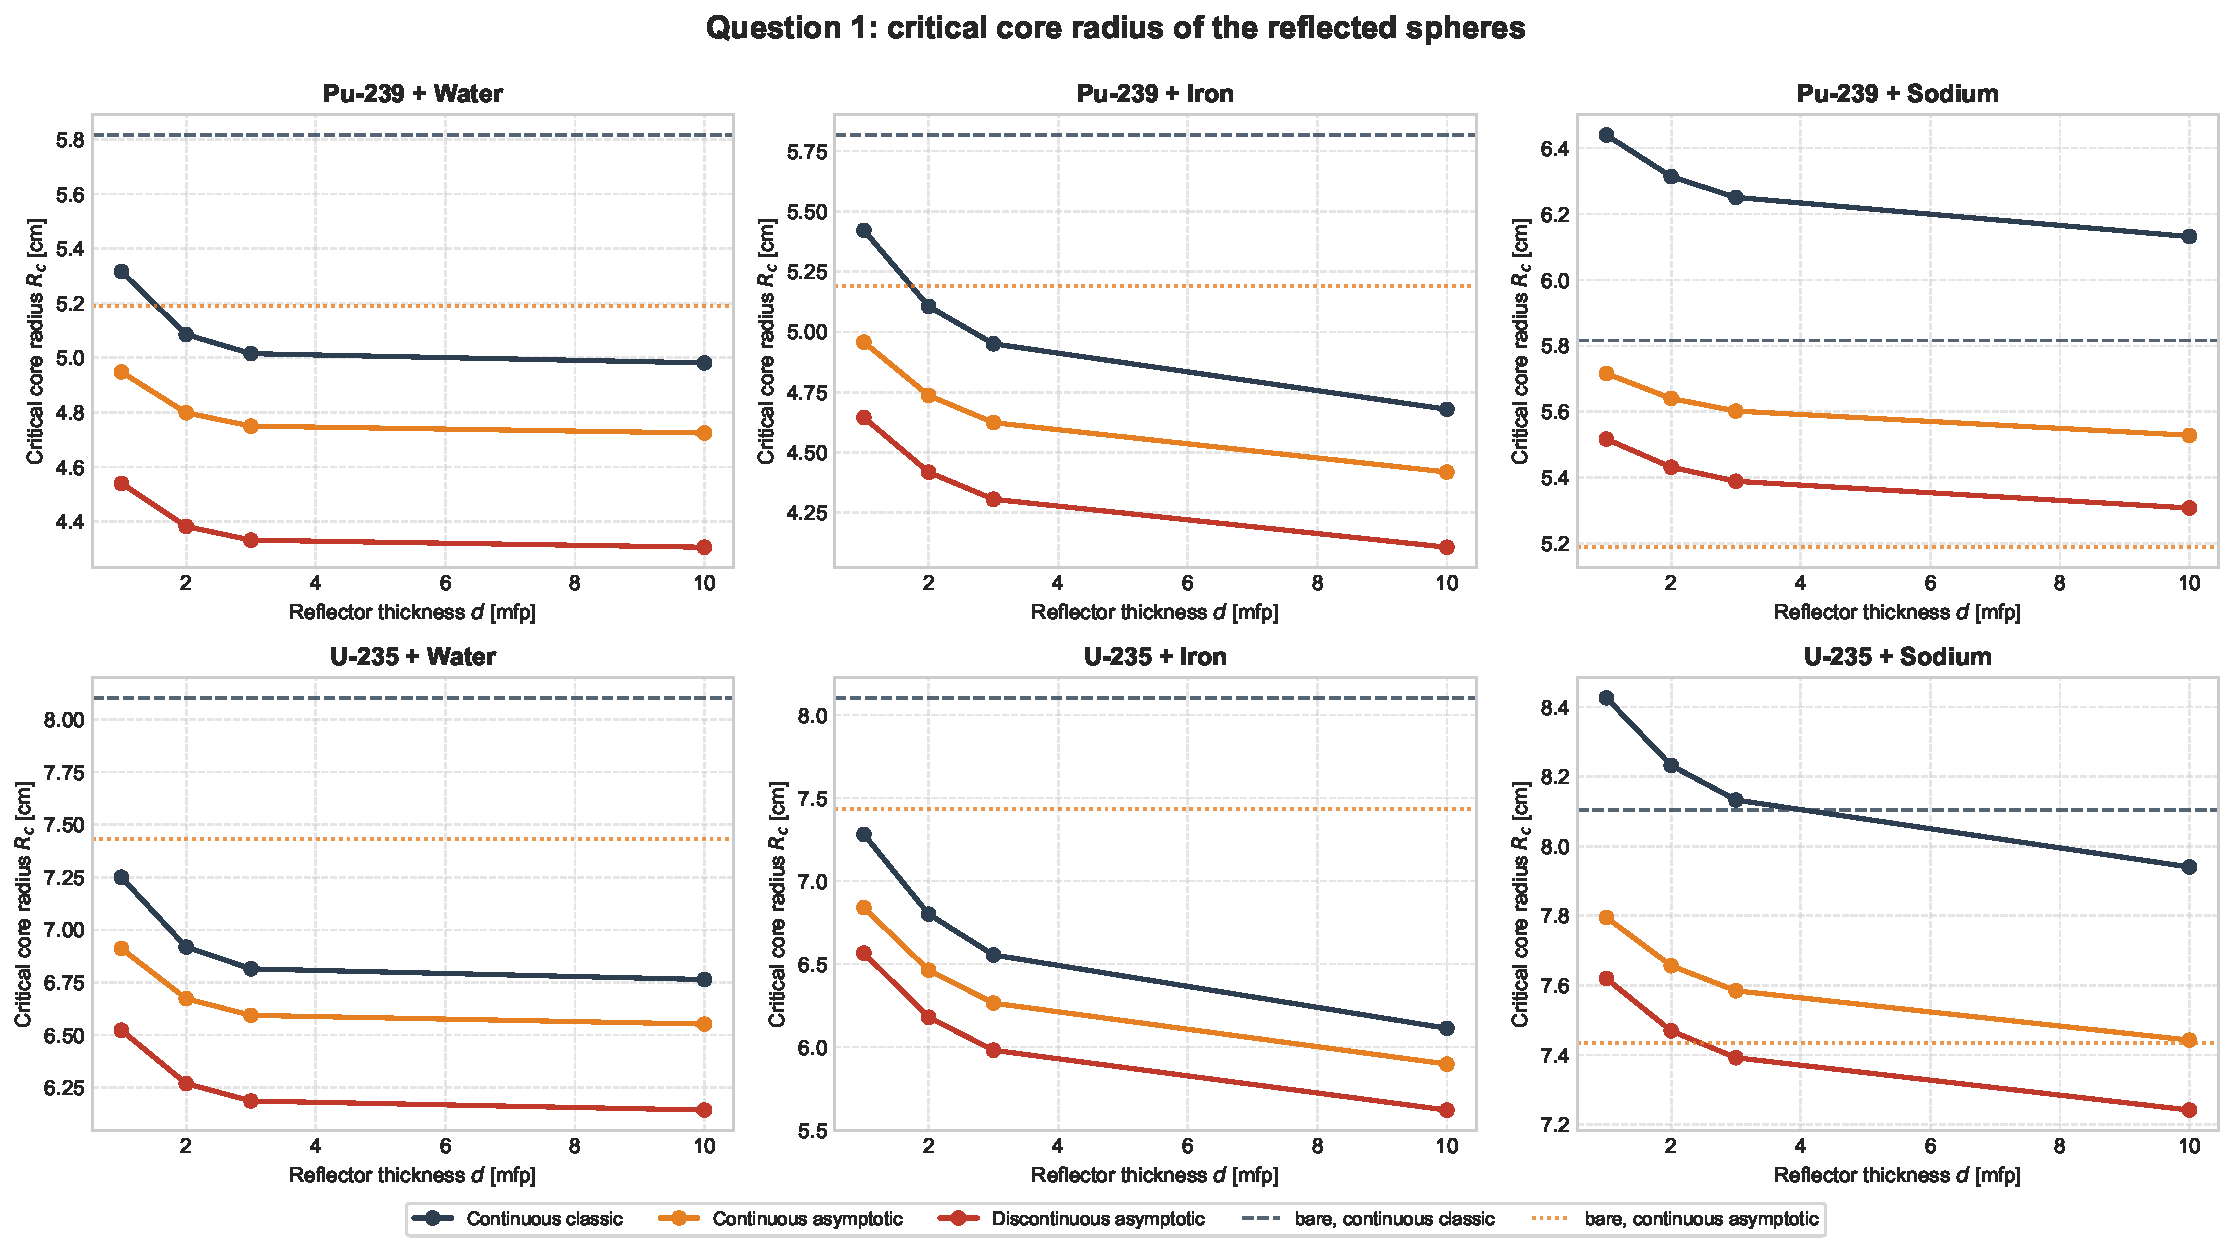
\includegraphics[width=\textwidth]{figs/q1_critical_radius.pdf}
\caption{Critical core radius against reflector optical thickness. Dashed and dotted lines are the two bare references. Water saturates by $d = 3$ mfp, iron is still improving at $d = 10$ mfp and the sodium (a) and (b) curves sit above their bare lines throughout, while (c) does not}.
\end{figure}

\begin{figure}[htbp]
\centering
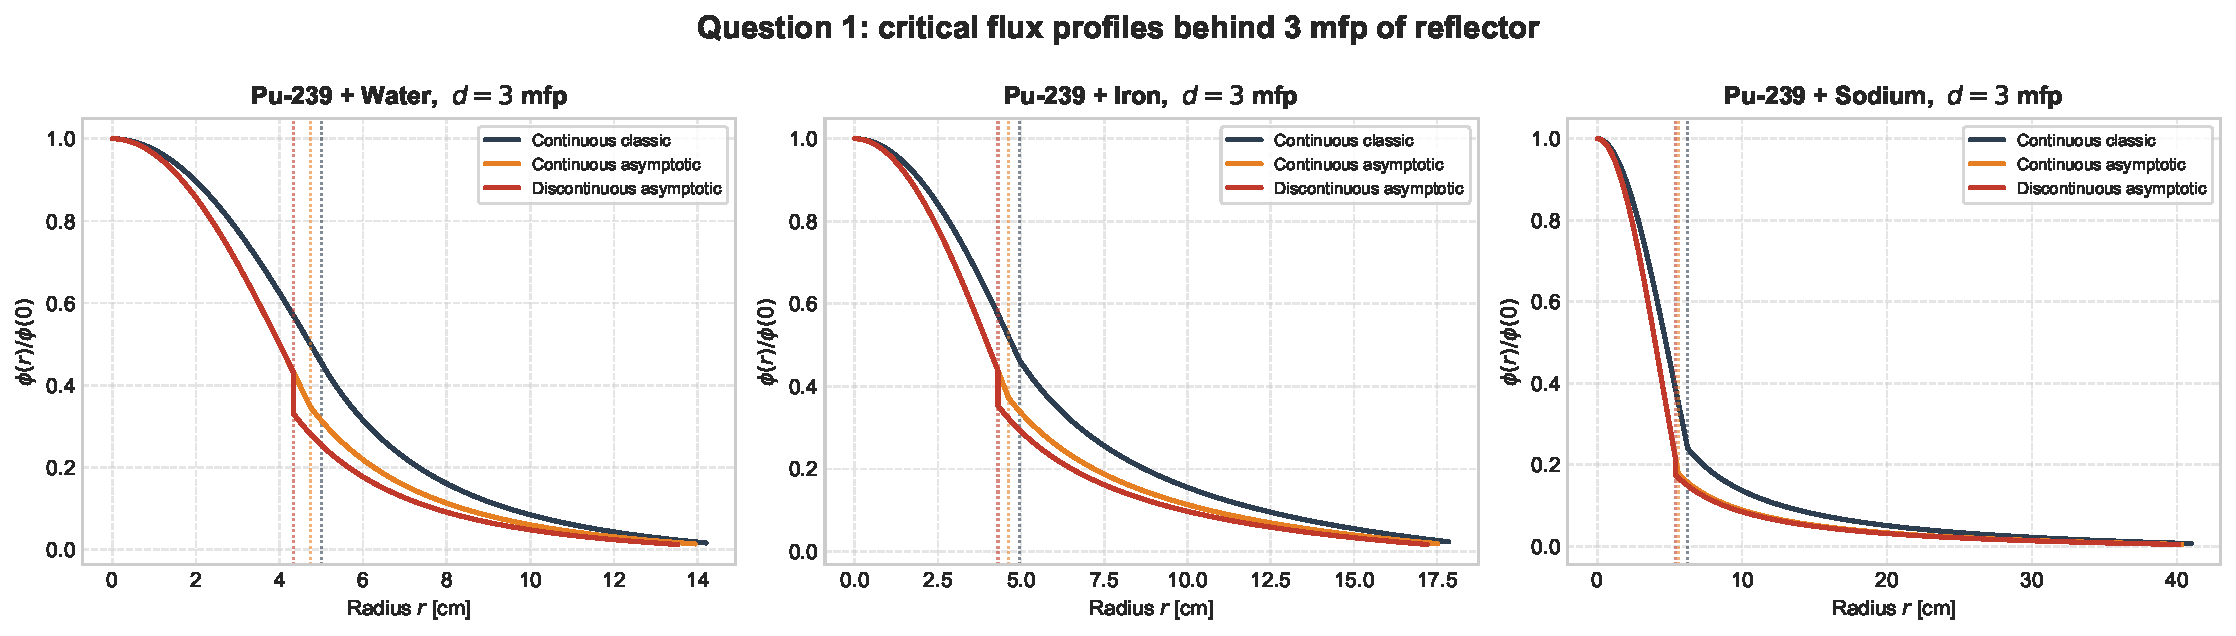
\includegraphics[width=\textwidth]{figs/q1_flux_profiles.pdf}
\caption{Critical flux across core and reflector for the Pu-239 core behind 3 mfp, normalised to $\phi(0)=1$. Dotted verticals mark each theory's interface. The discontinuous curve drops by the factor $\mu_0(c_R)/\mu_0(c_C)$ at the interface. Note the horizontal scale of the sodium panel, the wide one beneath: 3 mfp of sodium is 34.7 cm.}
\end{figure}


\begin{table}[htbp]
\centering
\begin{tabular}{lccccc}
\toprule
reflector & $D_R$ [cm] & shell [cm] & geometric $D_R/R_c$ & far-face $D_R/L$ & total vs.\ bare $0.5592$ \\
\midrule
Water  & 1.021 & 30.6  & 0.2050 & 0.1826 & 0.3876 \\
Iron   & 1.433 & 43.0  & 0.3063 & 0.0381 & 0.3444 \\
Sodium & 3.859 & 115.8 & \textbf{0.6295} & 0.0312 & 0.6607 \\
\bottomrule
\end{tabular}
\caption{Leakage ratio at the interface, in cm$^{-1}$, classic theory. Sodium's far-face return is the best of the three --- 10 mfp of a pure scatterer really does send almost everything back --- but its geometric term alone exceeds what a bare vacuum surface leaks.}
\end{table}

\FloatBarrier
\section*{Question 2: Critical slab half-thickness by $P_N$}

A homogeneous slab of total thickness $a$, reflective at the midplane $x=0$ and vacuum at
$x=a/2$, in mean free paths ($\Sigma_t=1$), for $c\in\{1.2,1.5,1.8\}$ and $N\in\{1,3,5,9\}$.
The unknown is the critical half-thickness $a/2$ at which $k_{\text{eff}}=1$ --- the same
quantity Question 3 tabulates for $S_N$, written the same way, so the two tables compare entry
by entry.

\subsection*{The $P_N$ equations}

Questions 2--5 all solve the same one-speed slab equation, written out as scattering and fission kept apart, and only the fission
source divided by $k$,
\begin{equation}
    \mu\frac{\partial \psi}{\partial x} + \Sigma_t\,\psi(x,\mu)
    = \frac{1}{2}\left[\Sigma_s\,\phi(x) + \frac{1}{k}\,\nu\Sigma_f\,\phi(x)\right] \label{eq:slab-eq}
\end{equation}
Since each one of the questions 2-4 specify only $c$ rather than giving $\Sigma_s$ and $\nu\Sigma_f$ separately, taking the free parameter to be $\Sigma_s=0$ causes $\nu\Sigma_f=c$ and puts the entire source under $k$, leaving an equation in $c$ alone:
\begin{equation}
    \mu\frac{\partial \psi}{\partial x} + \psi(x,\mu) = \frac{c}{2k}\,\phi_0(x),
    \qquad \phi_n(x) = \int_{-1}^{1} P_n(\mu)\,\psi(x,\mu)\,d\mu
    \label{eq:pntransport}
\end{equation}
\begin{notebox}[Explaining why $\Sigma_s$ can be chosen freely][blue]
This question fixes $\Sigma_t=1$ and $c=(\Sigma_s+\nu\Sigma_f)/\Sigma_t$ and
nothing else, so $\Sigma_s$ is a free parameter: every split $\nu\Sigma_f = c-\Sigma_s$ with
$0\le\Sigma_s\le c$ realises the stated $c$, and they are different media. The split cannot
change the quantity asked for, because at $k=1$ the bracket collapses to $\tfrac{c}{2}\phi$
whatever it is, so the critical half-thickness is \uline{a function of $c$ alone.} It does change $k$
at every other half-thickness --- $\Sigma_s$ is not divided by $k$ --- so $c$ alone fixes the
root of $k(a/2)-1$ but not $k(a/2)$ itself. 
\end{notebox}
Expanding $\psi(x,\mu)=\sum_{n^\prime\ge0}\frac{2n^\prime+1}{2}\phi_{n^\prime}(x)P_{n^\prime}(\mu)$, multiplying
\eqref{eq:pntransport} by $P_n(\mu)$ and integrating over $\mu$ turns the streaming term into
a three-term coupling through \uline{the Legendre recurrence}
$(2n+1)\mu P_n = (n+1)P_{n+1} + n P_{n-1}$, while the collision term is diagonal and the
isotropic source reaches only $n=0$:
\begin{equation}
    \frac{n+1}{2n+1}\frac{d\phi_{n+1}}{dx} + \frac{n}{2n+1}\frac{d\phi_{n-1}}{dx}
    + \phi_n(x) = \delta_{n0}\,\frac{c}{k}\,\phi_0(x),
    \qquad n=0,\dots,N
    \label{eq:pnrec}
\end{equation}
The system closes on itself once $\phi_{N+1}\equiv 0$ is imposed, which is the entire content
of the $P_N$ approximation (also notice that $\mathbf{\tilde A_{0,-1}=0}$ so this closure over the $N+1$ equations is handed for free). In vector form, with $\boldsymbol{\Phi}=(\phi_0,\dots,\phi_N)^{T}$,
\begin{equation}
    \mathbf{\tilde A}\,\frac{d\boldsymbol{\Phi}}{dx} + \mathbf{\Sigma}(k)\,\boldsymbol{\Phi} = 0,
    \qquad
    \tilde A_{n,n+1}=\frac{n+1}{2n+1},\quad \tilde A_{n,n-1}=\frac{n}{2n+1},
    \qquad
    \mathbf{\Sigma}_0(k)=\text{diag}\!\left(1-\tfrac{c}{k},1,\dots,1\right)
    \label{eq:pnmatrix}
\end{equation}
$\mathbf{\tilde A}$ is the Jacobi matrix of the Legendre recurrence truncated at order $N$, so
its $N+1$ eigenvalues are exactly the roots of $P_{N+1}(\mu)$ --- the Gauss--Legendre ordinates
of $S_{N+1}$. That is the algebraic content of the claim in Question 3 that the two methods share
their interior equations and differ only at the boundary.

\subsection*{Boundary conditions}

At the midplane ($x=0$) the flux is even in $\mu$, so every odd moment vanishes:
\begin{equation}
    \phi_{2m+1}(0) = 0, \qquad m=0,\dots,\tfrac{N-1}{2}
    \label{eq:pnsym}
\end{equation}
Equivalently $d\phi_{2m}/dx|_{0}=0$, which \eqref{eq:pnrec} then delivers for free (Notice that only one of
the two families may be imposed or the problem is over-determined.)s

At $x=a/2$ no neutron enters, $\psi(a/2,\mu)=0$ for $\mu<0$, which $N+1$ moments cannot satisfy
pointwise. Marshak's choice is to annihilate the $\tfrac{N+1}{2}$ lowest odd moments of the
incoming half-range,
\begin{equation}
    \int_{-1}^{0}\mu^{2m-1}\psi(\tfrac{a}{2},\mu)\,d\mu = 0
    \;\Longrightarrow\;
    \sum_{n=0}^{N} c_{mn}\,\phi_n(\tfrac{a}{2}) = 0,
    \qquad
    c_{mn} = \frac{2n+1}{2}\int_{-1}^{0}\mu^{2m-1}P_n(\mu)\,d\mu
    \label{eq:marshak}
\end{equation}
for $m=1,\dots,\tfrac{N+1}{2}$. The coefficients follow from
$P_n(-\mu)=(-1)^nP_n(\mu)$,
\begin{equation}
    c_{mn} = (-1)^{n+1}\,\frac{2n+1}{2}\int_{0}^{1}\mu^{2m-1}P_n(\mu)\,d\mu
\end{equation}
\begin{sloppypar}
whose integrand is a polynomial of degree at most $2N$, so an $(N+1)$-point Gauss--Legendre
rule mapped to $[0,1]$ evaluates it \uline{exactly} rather than approximately as done in \texttt{pn.algebra.marshak\_matrix}.
\end{sloppypar}

\uline{To sum up}, \eqref{eq:pnrec} is $N+1$ first-order equations and needs $N+1$ conditions.
\eqref{eq:pnsym} supplies $\tfrac{N+1}{2}$ and \eqref{eq:marshak} the other $\tfrac{N+1}{2}$.


\subsection*{Box discretisation and the Bell \& Glasstone $k$ iteration}

\paragraph{The scheme.} Divide $[0,a/2]$ into $J$ cells of width $\Delta x = a/(2J)$ with nodes
$x_j=j\Delta x$. Integrating \eqref{eq:pnmatrix} over one cell and closing it with the
midpoint rule --- derivative by the difference across the cell, value by the average of the
two faces ---
\begin{equation}
    \left.\frac{d\phi_n}{dx}\right|_{j+\frac12}\!\!\approx \frac{\phi_{n,j+1}-\phi_{n,j}}{\Delta x},
    \qquad
    \phi_{n,j+\frac12}\approx \frac{\phi_{n,j+1}+\phi_{n,j}}{2}
\end{equation}
gives one $(N+1)$-row block per cell,
\begin{equation}
    \left(\frac{\mathbf{\tilde A}}{\Delta x}+\frac{\mathbf{I}}{2}\right)\boldsymbol{\Phi}_{j+1}
    +\left(\frac{\mathbf{I}}{2}-\frac{\mathbf{\tilde A}}{\Delta x}\right)\boldsymbol{\Phi}_{j}
    = q_{j+\frac12}\,\mathbf{e}_0,
    \qquad j=0,\dots,J-1
    \label{eq:box}
\end{equation}

\paragraph{The linear system.} Stacking the $J+1$ nodal vectors gives $(J+1)(N+1)$ unknowns.
Equation \eqref{eq:box} supplies $J(N+1)$ rows, \eqref{eq:pnsym} supplies $\tfrac{N+1}{2}$ rows
acting on $\boldsymbol{\Phi}_0$ and \eqref{eq:marshak} the last $\tfrac{N+1}{2}$ acting on
$\boldsymbol{\Phi}_J$. the count closes exactly. Ordered node by node the matrix is
block-bidiagonal with two boundary blocks, i.e.\ banded with half-bandwidth $N+1$, and one
banded (or sparse) LU factorisation solves it. Call that matrix $\mathbf{L}$: it carries
streaming, collision and both boundary conditions, and it does \emph{not} depend on $k$.

\paragraph{The $k$ update.} Bell \& Glasstone update $k$ by the ratio of successive fission
productions,
\begin{equation}
    k^{(\ell+1)} = k^{(\ell)}\,
    {\frac{\displaystyle\int_0^{a/2} \frac{c\,\Sigma_t}{k^{(\ell)}}\,\phi_0^{(\ell+1)}\,dx}
                          {\displaystyle\int_0^{a/2} \frac{c\,\Sigma_t}{k^{(\ell)}}\,\phi_0^{(\ell)}\,dx}
    \;=\; k^{(\ell)}\,}
    \frac{\displaystyle\int_0^{a/2} \phi_0^{(\ell+1)}\,dx}
         {\displaystyle\int_0^{a/2} \phi_0^{(\ell)}\,dx}
    \label{eq:kupdate}
\end{equation}
The middle form is what the method actually compares: the fission source
\eqref{eq:box} that $\phi_0^{(\ell+1)}$ would build against the one that produced it, so it is
an exact ratio of sources and not of fluxes that happen to resemble them. The iterate is then rescaled by $\max_j\phi_{0,j}$, which
has no effect on \eqref{eq:kupdate} --- it only keeps the vector from drifting towards $0$ or
$\infty$ as $k^{\ell}$ compounds --- and the loop stops on $|k^{(\ell+1)}-k^{(\ell)}|<\epsilon_k$.
Convergence is linear at the dominance ratio of the two leading eigenvalues, which for a bare
slab is well separated, and the starting guess
\begin{equation}
    \phi_0^{(0)}(x)=\cos\!\left(\frac{\pi x}{2\,(a/2+0.7104)}\right),\qquad k^{(0)}=1
\end{equation}
is the diffusion fundamental mode with the asymptotic extrapolation distance, already almost
the answer.

\paragraph{The outer loop.} Dividing the fission source by $k$ makes a solution exist at every
thickness, so criticality is a root search on
\begin{equation}
    f(a/2) = k(a/2) - 1
\end{equation}


\begin{algorithm}[H]
\caption{Critical half-thickness by the box $P_N$ scheme --- \texttt{homework3.pn.box}}
\label{alg:pnbox}
\KwIn{secondaries $c$, order $N$, cells $J$, initial guess $(a/2)_0$}
\KwOut{$(a/2)_{\text{crit}}$ such that $k=1$}
\Fn{\BoxSystem{$a/2$, medium, $N$, $J$}}{
  \tcc{Setup -- once per $(a/2,N)$, outside every loop}
  $\Delta x \leftarrow (a/2)/J$\;
  assemble $\mathbf{L}$ of order $(J+1)(N+1)$: $\tfrac{N+1}{2}$ symmetry rows
    \eqref{eq:pnsym} on $\boldsymbol{\Phi}_0$; $J$ cell blocks \eqref{eq:box}; $\tfrac{N+1}{2}$
    Marshak rows \eqref{eq:marshak} on $\boldsymbol{\Phi}_J$\;
  \KwRet{\Splu{$\mathbf{L}$}}
    \tcp*{\textbf{factorise once}; banded, half-bandwidth $N+1$}
}
\BlankLine
\Fn{\KEig{$a/2$, medium, $N$, $J$}}{
  system $\leftarrow$ \BoxSystem{$a/2$, medium, $N$, $J$}
    \tcp*{the only factorisation}
  $\phi_0 \leftarrow \cos\!\left(\pi x / 2(a/2+0.7104)\right)$,\quad $k \leftarrow 1$\;
  \tcc{Power iteration (Bell \& Glasstone)}
  \Repeat{$|k_{\text{new}}-k| < \epsilon_k\,|k_{\text{new}}|$}{
    $q \leftarrow \dfrac{c\,\Sigma_t}{k}\,\Midpoints{$\phi_0$}$, in the $\phi_0$ row of each
      cell block \tcp*{$\phi$ stage}
    $\boldsymbol{\Phi} \leftarrow \BoxSolve{$q$}$
      \tcp*{\textbf{two substitutions, no refactorisation}}
    $\phi_0^{\text{new}} \leftarrow$ moment $n=0$ of $\boldsymbol{\Phi}$\;
    $k_{\text{new}} \leftarrow k\,\dfrac{\sum \Midpoints{$\phi_0^{\text{new}}$}}
                                        {\sum \Midpoints{$\phi_0$}}$
      \tcp*{$k$ stage, eq.~\eqref{eq:kupdate}}
    $\phi_0 \leftarrow \phi_0^{\text{new}} / \max_j \phi^{\text{new}}_{0,j}$,\quad
      $k \leftarrow k_{\text{new}}$ \tcp*{rescale: keeps $k^\ell$ from compounding}
  }
  \KwRet{$k$}
}
\BlankLine
\tcc{critical\_half\_thickness, which defers to sn.core}
\KwRet{\CritSize{$a/2 \mapsto \KEig{a/2}-1$, $(a/2)_0$}}
\end{algorithm}

\begin{sloppypar}
Every name in Algorithm~\ref{alg:pnbox} is the identifier the code uses.
\texttt{BoxSystem} is the constructor \texttt{pn.box.BoxSystem.\_\_init\_\_}, \texttt{splu} is
\texttt{scipy.sparse.linalg.splu} applied to the CSC form, and \texttt{critical\_size} is
borrowed from \texttt{sn.core} --- the one place Question 2 reuses the $S_N$ package.
\end{sloppypar}

\paragraph{Errors.} The box scheme is second order, so the discretisation error in
$(a/2)_{\text{crit}}$ falls as $\Delta x^2$ and is separable from the truncation error in $N$ by
running the same $N$ on a refined mesh --- the check reported in Question 3 for $S_N$.


\FloatBarrier
\subsection*{Results}

\begin{table}[htbp]
\centering
\begin{tabular}{ccccc}
\toprule
$c$ & order & $(a/2)_{\text{crit}}$ [mfp] & exact transport [mfp] & departure \\
\midrule
1.2 & $P_1$ & 1.412502 & 1.28981 & $+9.51\%$ \\
1.2 & $P_3$ & 1.302001 & 1.28981 & $+0.95\%$ \\
1.2 & $P_5$ & 1.292597 & 1.28981 & $+0.22\%$ \\
1.2 & $P_9$ & 1.290382 & 1.28981 & $+0.04\%$ \\
\midrule
1.5 & $P_1$ & 0.723480 & 0.60762 & $+19.07\%$ \\
1.5 & $P_3$ & 0.629149 & 0.60762 & $+3.54\%$ \\
1.5 & $P_5$ & 0.612136 & 0.60762 & $+0.74\%$ \\
1.5 & $P_9$ & 0.606467 & 0.60762 & $-0.19\%$ \\
\midrule
1.8 & $P_1$ & 0.496560 & 0.39314 & $+26.31\%$ \\
1.8 & $P_3$ & 0.418210 & 0.39314 & $+6.38\%$ \\
1.8 & $P_5$ & 0.399736 & 0.39314 & $+1.68\%$ \\
1.8 & $P_9$ & 0.391130 & 0.39314 & $-0.51\%$ \\
\bottomrule
\end{tabular}
\caption{Critical half-thickness $(a/2)_{\text{crit}}$ in mean free paths, by the box scheme on
200 cells. The departure is measured against the exact-transport reference
$a/2 = \tfrac{\pi}{2}\nu_0 - z_0$ of Assignment 1.}
\end{table}

\begin{figure}[htbp]
\centering
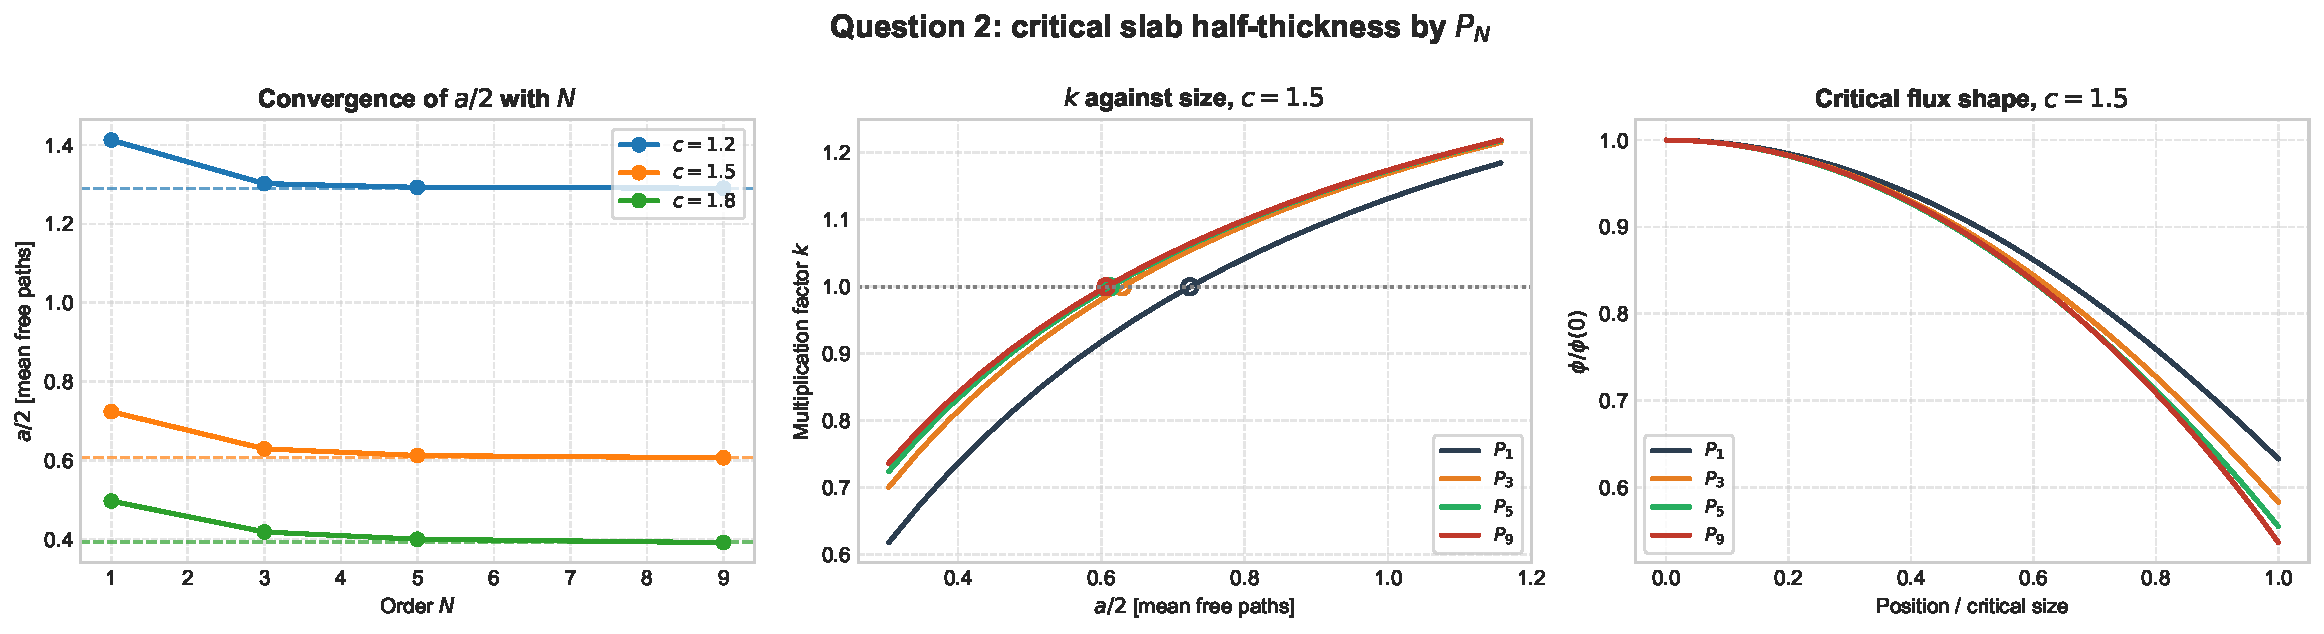
\includegraphics[width=\textwidth]{figs/q2_pn_slab_orders.pdf}
\caption{Top left: convergence of $(a/2)_{\text{crit}}$ with $N$, dashed lines the
exact-transport values. Top right: $k$ against half-thickness at $c=1.5$, circles the $k=1$
crossings, which for $P_3$, $P_5$ and $P_9$ are already almost on top of one another. Beneath
them: the normalised critical flux --- as in Question 3, the order changes the surface value
and not the interior shape.}
\end{figure}

\FloatBarrier
\section*{The $S_N$ method of Questions 3--5}

All three questions solve the same monoenergetic, steady-state problem,
\begin{equation}
    \mu \frac{\partial \psi}{\partial x} + \Sigma_t \psi = \frac{1}{2}\left[\Sigma_s \phi + \frac{1}{k}\nu\Sigma_f \phi\right],
    \qquad \phi(x) = \int_{-1}^{1}\psi(x,\mu)\,d\mu
    \label{eq:snbase}
\end{equation}
with the same three ingredients: a Gauss--Legendre quadrature in angle, diamond differencing in space with a negative-flux fixup, and the Bell \& Glasstone $k$ iteration. Lengths are mean free paths in Questions 3 and 4 and centimetres in Question 5.

\paragraph{Angle.} The $N$ ordinates $\{\mu_m\}$ and weights $\{w_m\}$ are the Gauss--Legendre nodes on $[-1,1]$, so that $\mu_{N-m+1}=-\mu_m$, $\sum_m w_m = 2$, and
\begin{equation}
    \phi_i = \sum_{m=1}^{N} w_m \psi_{i,m}
\end{equation}

\paragraph{Space, slab.} The slab equation is \eqref{eq:snbase} at ordinate $m$,
$\mu_m \partial \psi_m/\partial x + \Sigma_t \psi_m = S/2$, whose conservative form
integrates over the cell $x\in[x_{i-1/2},x_{i+1/2}]$ to
\begin{equation}
    \mu_m\left(\psi_{i+\frac12,m} - \psi_{i-\frac12,m}\right)
    + \Sigma_t \Delta x\, \psi_{i,m} = \frac{S_i}{2}\Delta x
    \label{eq:slabbalance}
\end{equation}
with the diamond closure $\psi_{i,m} = \tfrac12\left(\psi_{i+1/2,m}+\psi_{i-1/2,m}\right)$
relating the cell centre to its two faces. Which face is the outflow depends on the sign of
$\mu_m$, and that is the whole of the difference between the two sweeps.

\textcolor{blue}{\emph{Forward sweep}, $\mu_m>0$: the flux enters at $x_{i-1/2}$ and leaves at
$x_{i+1/2}$, so the closure is used as $\psi_{i+1/2,m}=2\psi_{i,m}-\psi_{i-1/2,m}$. Substituting
it into \eqref{eq:slabbalance} removes the outgoing face,}
\begin{equation}
    \mu_m\left(2\psi_{i,m}-2\psi_{i-\frac12,m}\right) + \Sigma_t \Delta x\,\psi_{i,m}
    = \frac{S_i}{2}\Delta x
\end{equation}
\textcolor{blue}{and collecting $\psi_{i,m}$ gives the cell centre and then, from the closure
again, the flux handed to the next cell $i+1$:}
\begin{equation}
    \psi_{i,m} = \frac{\tfrac12 S_i \Delta x + 2\mu_m\,\psi_{i-\frac12,m}}
                      {\Sigma_t \Delta x + 2\mu_m},
    \qquad
    \psi_{i+\frac12,m} = 2\psi_{i,m} - \psi_{i-\frac12,m}
    \label{eq:slabsweep}
\end{equation}
\textcolor{blue}{marched from $x=0$ outwards, starting from the reflected flux there.}

\textcolor{blue}{\emph{Backward sweep}, $\mu_m<0$: the roles swap. Writing $\mu_m=-|\mu_m|$ turns
the leading term of \eqref{eq:slabbalance} into
$|\mu_m|(\psi_{i-1/2,m}-\psi_{i+1/2,m})$, so the flux enters at $x_{i+1/2}$ and leaves at
$x_{i-1/2}$, and the closure is used the other way round,
$\psi_{i-1/2,m}=2\psi_{i,m}-\psi_{i+1/2,m}$:}
\begin{equation}
    \psi_{i,m} = \frac{\tfrac12 S_i \Delta x + 2|\mu_m|\,\psi_{i+\frac12,m}}
                      {\Sigma_t \Delta x + 2|\mu_m|},
    \qquad
    \psi_{i-\frac12,m} = 2\psi_{i,m} - \psi_{i+\frac12,m}
    \label{eq:slabsweepback}
\end{equation}
\textcolor{blue}{marched from the vacuum face at $x=a/2$ inwards, starting from
$\psi_{I+1/2,m}=0$. The two are the same formula with the inflow face exchanged, which is why
one $|\mu_m|$ serves both.}

\paragraph{Space, sphere.} The spherical equation carries an angular redistribution term, that can be seen in Eq. (2.46) in Pomraning's book (pg. 30):
\begin{equation}
    \mu \frac{\partial \psi}{\partial r} + \frac{1-\mu^2}{r}\frac{\partial \psi}{\partial \mu} + \Sigma_t \psi = \frac{S}{2}
\end{equation}
whose conservative form integrates over the cell $(r,\mu)\in[r_{i-1/2}, r_{i+1/2}]\times[\mu_{m-1/2}, \mu_{m+1/2}]$ to
\begin{equation}
    \mu_m\left(A_{i+\frac12}\psi_{i+\frac12,m} - A_{i-\frac12}\psi_{i-\frac12,m}\right)
    + \beta_{i,m}\left(\alpha_{m+\frac12}\psi_{i,m+\frac12} - \alpha_{m-\frac12}\psi_{i,m-\frac12}\right)
    + \Sigma_t V_i \psi_{i,m} = \frac{S_i}{2}V_i
    \label{eq:sphbalance}
\end{equation}
with $A = 4\pi r^2$, $V_i = \tfrac{4\pi}{3}(r_{i+1/2}^3 - r_{i-1/2}^3)$ and the area increment
$\beta_{i,m} = \left(A_{i+1/2}-A_{i-1/2}\right)/w_m$. The angular coefficients follow from demanding that a flat flux solve \eqref{eq:sphbalance} exactly:
\begin{equation}
    \alpha_{\frac12} = 0, \qquad \alpha_{m+\frac12} = \alpha_{m-\frac12} - w_m \mu_m,
    \qquad \alpha_{N+\frac12} = 0 \ \text{ since } \sum_m w_m \mu_m = 0
\end{equation}
The recursion needs a starting value $\psi_{i,1/2}$ at $\mu_{1/2}=-1$, where $1-\mu^2=0$ and the angular derivative drops out; what remains, $-\partial \psi/\partial r + \Sigma_t \psi = S/2$, is \eqref{eq:slabsweepback} at $|\mu|=1$, run inwards from the vacuum boundary.

\textcolor{blue}{\paragraph{The two faces of a spherical cell.} Equation \eqref{eq:sphbalance} is
\eqref{eq:slabbalance} with a second outgoing face. They are not alike and it is worth naming
them separately:}
\begin{itemize}
    \item \textcolor{blue}{the \emph{radial face}, weighted by the two shell areas
    $A_{i\pm1/2}$, whose outflow feeds the \textbf{next radial cell} of the same ordinate.
    Which of the two areas is the outflow depends on the sign of $\mu_m$, exactly as in the
    slab;}
    \item \textcolor{blue}{the \emph{angular face}, weighted by the two coefficients
    $\alpha_{m\pm1/2}$ of the angular bin, whose outflow feeds the \textbf{next ordinate} in
    the same cell. This one never swaps: $d\mu/ds\ge0$ means $\mu$ only increases, so the
    inflow is always at $m-\tfrac12$ and the outflow always at $m+\tfrac12$.}
\end{itemize}
\textcolor{blue}{Each closes with its own diamond relation,}
\begin{align}
    \psi_{i+\frac12,m} &= 2\psi_{i,m} - \psi_{i-\frac12,m}
        \quad (\mu_m>0), \qquad
    \psi_{i-\frac12,m} = 2\psi_{i,m} - \psi_{i+\frac12,m} \quad (\mu_m<0)
        \label{eq:closr} \\
    \psi_{i,m+\frac12} &= 2\psi_{i,m} - \psi_{i,m-\frac12}
        \label{eq:closmu}
\end{align}

\textcolor{blue}{Take the forward sweep, $\mu_m>0$, so that the radial outflow is
$A_{\text{out}}=A_{i+1/2}$ and the inflow $A_{\text{in}}=A_{i-1/2}$. Substituting
\eqref{eq:closr} and \eqref{eq:closmu} into \eqref{eq:sphbalance} eliminates both outgoing
fluxes at once:}
\begin{multline}
    \mu_m\left(2A_{\text{out}}\psi_{i,m} - \left(A_{\text{out}}+A_{\text{in}}\right)\psi_{i-\frac12,m}\right) \\
    + \beta_{i,m}\left(2\alpha_{m+\frac12}\psi_{i,m} - \left(\alpha_{m+\frac12}+\alpha_{m-\frac12}\right)\psi_{i,m-\frac12}\right)
    + \Sigma_t V_i \psi_{i,m} = \frac{S_i}{2}V_i
    \label{eq:sphcollect}
\end{multline}
\textcolor{blue}{Every term now carries either $\psi_{i,m}$ or a known inflow, so collecting
$\psi_{i,m}$ on the left gives the cell solve outright:}
\begin{equation}
    \boxed{\;
    \psi_{i,m} = \frac{\tfrac12 S_i V_i
        + \mu_m\left(A_{\text{out}}+A_{\text{in}}\right)\psi_{i-\frac12,m}
        + \beta_{i,m}\left(\alpha_{m+\frac12}+\alpha_{m-\frac12}\right)\psi_{i,m-\frac12}}
        {\Sigma_t V_i + 2\mu_m A_{\text{out}} + 2\beta_{i,m}\alpha_{m+\frac12}}\;}
    \label{eq:cellflux}
\end{equation}
\textcolor{blue}{and \eqref{eq:closr} and \eqref{eq:closmu} then hand on the two fluxes the
march needs next --- $\psi_{i+1/2,m}$ to radial cell $i+1$, and $\psi_{i,m+1/2}$ to ordinate
$m+1$. The backward sweep is \eqref{eq:cellflux} with $A_{\text{out}}=A_{i-1/2}$,
$A_{\text{in}}=A_{i+1/2}$, $\mu_m$ replaced by $|\mu_m|$ and the radial inflow taken as
$\psi_{i+1/2,m}$; the angular half of the formula is untouched. Setting
$A_{\text{out}}=A_{\text{in}}=1$, $V_i=\Delta x$ and $\alpha_{m\pm1/2}=0$ returns
\eqref{eq:slabsweep} exactly, which is the check that the two cell solves are the same
balance. \textbf{In code they are kept apart on purpose: \texttt{sn.slab.cell\_flux} takes one
inflow, \texttt{sn.sphere.cell\_flux} takes a \texttt{radial\_face} and an
\texttt{angular\_face}.}}


\paragraph{Fixup.} Whenever a diamond outgoing flux $2\psi_{i,m}-\psi_{\text{in}}$ of \eqref{eq:closr} or \eqref{eq:closmu} comes out negative it is set to zero and the cell balance is re-solved with it held there, in angle as well as in space. Frankly, this never occurs in Questions 3--5: the fission source is proportional to the flux itself, so no cell is ever starved, and a critical system is thin enough that $\Sigma_t \Delta x / |\mu_m| < 2$ at every ordinate.

\paragraph{Boundary conditions.} Reflective at the symmetry point, $\psi_{1/2,m} = \psi_{1/2,m'}$ with $\mu_{m'}=-\mu_m$; vacuum at the outer face, $\psi_{I+1/2,m}=0$ for $\mu_m<0$.

\paragraph{Eigenvalue.} Outer iteration $l$ fixes the fission source $Q_{f,i}^{(l)} = \nu\Sigma_{f,i}\phi_i^{(l)}/k^{(l)}$; inner iteration $n$ sweeps $S_i = \Sigma_{s,i}\phi_i^{(n)} + Q_{f,i}^{(l)}$ until $\phi$ settles; then
\begin{equation}
    k^{(l+1)} = k^{(l)}\,\frac{P^{(l+1)}}{P^{(l)}},
    \qquad P^{(l)} = \sum_i \nu\Sigma_{f,i}\,\phi_i^{(l)}\,V_i
\end{equation}
Dividing the fission source by $k$ makes a solution exist at \emph{every} system size, so criticality becomes a root search: \texttt{brentq} on $k(\text{size})-1$, which costs 8 evaluations of $k$.


{\color{blue}
\begin{algorithm}[H]
\caption{One transport solve --- backward ordinates, then forward ones ---
         \texttt{homework3.sn.slab} / \texttt{homework3.sn.sphere}}
\label{alg:sweep}
\KwIn{isotropic source $S_i$}
\KwOut{scalar flux $\phi_i$}
\KwData{$\psi_{\cdot,m-\frac12}$, the \emph{angular inflow column} --- one value per spatial
  cell, the half-angle flux ordinate $m$ consumes through its angular face. Sweeping $m$
  replaces it with $\psi_{\cdot,m+\frac12}$, which ordinate $m+1$ consumes in turn
  (\texttt{psi\_low} and \texttt{psi\_high} in the code). The slab has no such column.}
\Fn{\SweepAll{$S$}}{
  $q_i \leftarrow S_i/2$\;
  \lIf{sphere}{$\psi_{\cdot,\frac12} \leftarrow \StartDir{$q$}$
    \tcp*[f]{$\mu_{1/2}=-1$: no angular term, a plane march}}
  $\phi \leftarrow 0$;\quad $\psi_{\frac12,\cdot} \leftarrow 0$
    \tcp*{the reflective face, one value per ordinate}
  \For{$m$ \textnormal{with} $\mu_m<0$, \textnormal{ascending}}{
    $\psi_{\cdot,m},\ \psi_{\cdot,m+\frac12},\ \psi_{\frac12,m'} \leftarrow
      \SweepBack{$m$, $q$, $\psi_{\cdot,m-\frac12}$}$, \quad $\mu_{m'}=-\mu_m$\;
    $\phi \leftarrow \phi + w_m\,\psi_{\cdot,m}$\;
  }
  \For{$m$ \textnormal{with} $\mu_m>0$, \textnormal{ascending}}{
    $\psi_{\cdot,m},\ \psi_{\cdot,m+\frac12} \leftarrow
      \SweepFwd{$m$, $q$, $\psi_{\cdot,m-\frac12}$, $\psi_{\frac12,m}$}$
      \tcp*{starts from what $-\mu_m$ reflected}
    $\phi \leftarrow \phi + w_m\,\psi_{\cdot,m}$\;
  }
  \KwRet{$\phi$}
}
\BlankLine
\Fn{\SweepBack{$m$, $q$, $\psi_{\cdot,m-\frac12}$}}{
  $\psi_{\text{in}} \leftarrow 0$ \tcp*{vacuum: nothing enters the outer face}
  \For{$i \leftarrow I$ \KwTo $1$ \textnormal{(inwards)}}{
    \lIf{slab}{$\psi_{i,m},\,\psi_{\text{in}} \leftarrow
      \CellSlab{$\Sigma_t\Delta x$, $\tfrac12 S_i\Delta x$, $|\mu_m|$, $\psi_{\text{in}}$}$
      \tcp*[f]{eq.~\eqref{eq:slabsweepback}}}
    \lElse{$\psi_{i,m},\,\psi_{\text{in}},\,\psi_{i,m+\frac12} \leftarrow
      \CellSph{$\Sigma_tV_i$, $\tfrac12 S_iV_i$, radial\_face, angular\_face}$
      \tcp*[f]{eq.~\eqref{eq:cellflux}}}
  }
  \KwRet{$\psi_{\cdot,m}$, $\psi_{\cdot,m+\frac12}$, $\psi_{\text{in}}$}
    \tcp*{the last $\psi_{\text{in}}$ is what reflects at the centre}
}
\BlankLine
\Fn{\SweepFwd{$m$, $q$, $\psi_{\cdot,m-\frac12}$, $\psi_{\text{in}}$}}{
  \For{$i \leftarrow 1$ \KwTo $I$ \textnormal{(outwards)}}{
    the same cell solve, with the radial inflow and outflow faces exchanged
      \tcp*{eq.~\eqref{eq:slabsweep}}
  }
  \KwRet{$\psi_{\cdot,m}$, $\psi_{\cdot,m+\frac12}$}
}
\BlankLine
\tcc{The radial face swaps with the sign of $\mu_m$; the angular face never does --- its
     inflow is always $\psi_{i,m-1/2}$ and its outflow always $\psi_{i,m+1/2}$.}
\end{algorithm}
}

% This one floats rather than taking [H]: it does not fit under Algorithm 2, and [H] would
% place it anyway and overrun the footer. The \color is inside the float, not around it --
% a float is shipped out after an enclosing colour group has closed and would come out black.
\begin{algorithm}[tbp]
\color{blue}
\caption{The two iterations --- scattering inside, Bell \& Glasstone outside ---
         \texttt{homework3.sn.core}}
\label{alg:snk}
\KwIn{medium, geometry, initial guess $\text{size}_0$}
\KwOut{critical size}
\Fn{\RunSn{solver, medium, $Q_f$, $\phi$}}{
  \Repeat{$\max_i|\phi^{\text{new}}_i-\phi_i| \le \epsilon_\phi \max_i \phi^{\text{new}}_i$
          \textnormal{\ \ or\ } $\Sigma_s=0$}{
    $\phi^{\text{new}} \leftarrow \SweepAll{$\Sigma_s\phi + Q_f$}$
      \tcp*{one double sweep per inner}
  }
  \KwRet{$\phi$} \tcp*{$\Sigma_s=0$ (Q3, Q4): one sweep is already exact}
}
\BlankLine
\Fn{\KEig{solver}}{
  $\phi \leftarrow 1$;\quad $k \leftarrow 1$;\quad
    $P \leftarrow \sum_i \nu\Sigma_{f,i}\,\phi_i V_i$\;
  \Repeat{$|k_{\text{new}}-k| < \epsilon_k |k_{\text{new}}|$}{
    $\phi^{\text{new}} \leftarrow \RunSn{$\nu\Sigma_f \phi / k$}$
      \tcp*{$\phi$ iteration}
    $P^{\text{new}} \leftarrow \sum_i \nu\Sigma_{f,i}\,\phi^{\text{new}}_i V_i$\;
    $k_{\text{new}} \leftarrow k\,P^{\text{new}}/P$ \tcp*{$k$ iteration}
    $\phi \leftarrow \phi^{\text{new}}/\max_i\phi^{\text{new}}_i$ \tcp*{rescale, $P$ likewise}
  }
  \KwRet{$k$}
}
\BlankLine
\Fn{\CritSize{$k$ of size, $\text{size}_0$}}{
  widen a bracket about $\text{size}_0$ by $3\%$ a step until $\KEig{}-1$ changes sign\;
  \KwRet{\Brentq{$\text{size} \mapsto \KEig{size}-1$}}
}
\end{algorithm}

\begin{sloppypar}
\textcolor{blue}{Every name in Algorithms~\ref{alg:sweep} and~\ref{alg:snk} is the identifier
the code uses. \texttt{sweep\_backward}, \texttt{sweep\_forward},
\texttt{sweep\_all\_angles} and
\texttt{\_starting\_direction} are methods of \texttt{sn.slab.SlabSolver} and
\texttt{sn.sphere.SphereSolver} --- the two geometries supply them independently, which is why
everything in \texttt{sn.core} is written against neither. Three nested loops, and not one
matrix among them.}
\end{sloppypar}

\FloatBarrier
\section*{Question 3: Critical slab half-thickness by $S_N$}

Reflective at $x=0$, vacuum at $x=a/2$, 200 cells. The reference column is Assignment 1's exact-transport relation $a/2 = \tfrac{\pi}{2}\nu_0 - z_0$, evaluated from Case's tabulated $\nu_0$ and $z_0$.

\begin{table}[htbp]
\centering
\begin{tabular}{ccccc}
\toprule
$c$ & order & $a/2$ [mfp] & exact transport [mfp] & departure \\
\midrule
1.2 & $S_2$    & 1.48499 & 1.28981 & $+15.13\%$ \\
1.2 & $S_4$    & 1.31855 & 1.28981 & $+2.23\%$ \\
1.2 & $S_6$    & 1.29861 & 1.28981 & $+0.68\%$ \\
1.2 & $S_{10}$ & 1.29218 & 1.28981 & $+0.18\%$ \\
\midrule
1.5 & $S_2$    & 0.78001 & 0.60762 & $+28.37\%$ \\
1.5 & $S_4$    & 0.64949 & 0.60762 & $+6.89\%$ \\
1.5 & $S_6$    & 0.62089 & 0.60762 & $+2.18\%$ \\
1.5 & $S_{10}$ & 0.60904 & 0.60762 & $+0.23\%$ \\
\midrule
1.8 & $S_2$    & 0.54291 & 0.39314 & $+38.09\%$ \\
1.8 & $S_4$    & 0.43875 & 0.39314 & $+11.60\%$ \\
1.8 & $S_6$    & 0.41014 & 0.39314 & $+4.32\%$ \\
1.8 & $S_{10}$ & 0.39459 & 0.39314 & $+0.37\%$ \\
\bottomrule
\end{tabular}
\caption{Critical half-thickness in mean free paths. The departure is entirely angular: the same radii are reproduced to seven digits on meshes from 50 to 800 cells.}
\end{table}

\begin{figure}[htbp]
\centering
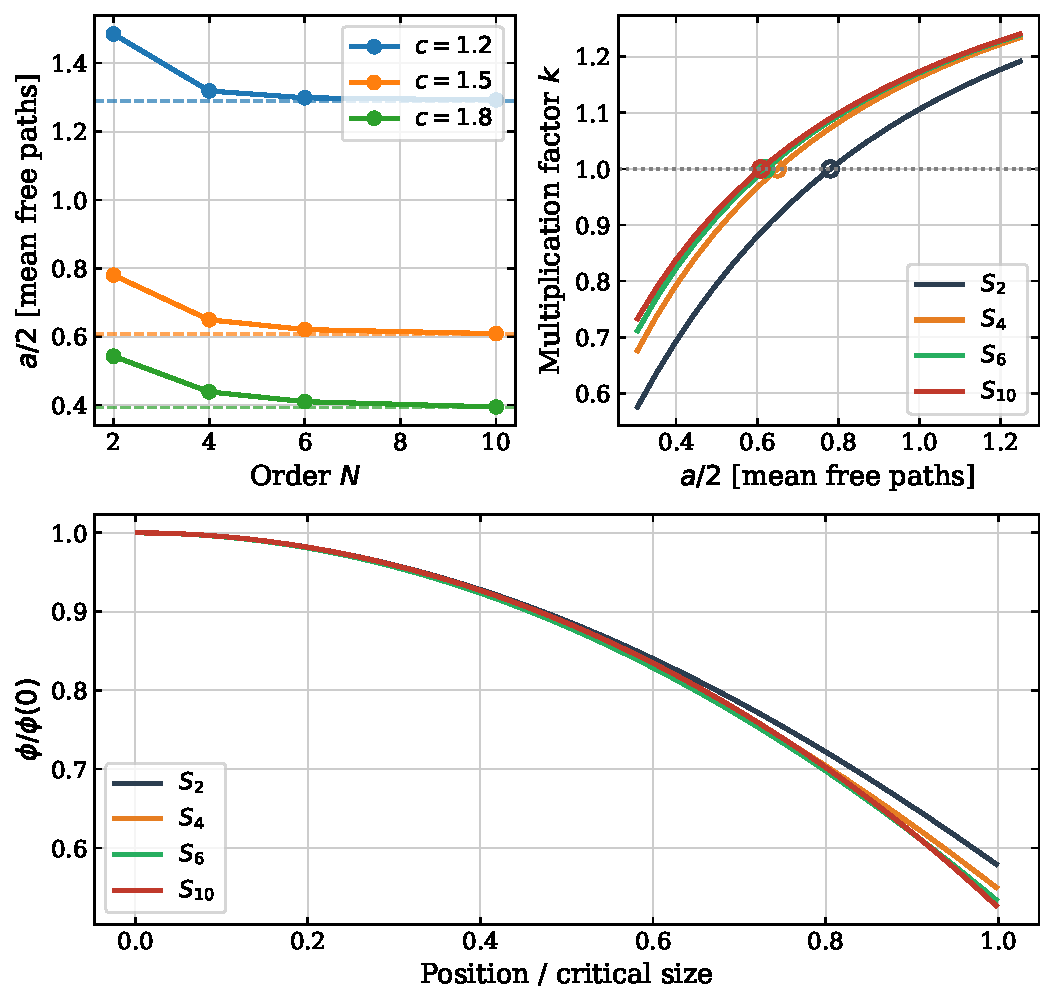
\includegraphics[width=\textwidth]{figs/q3_slab_orders.pdf}
\caption{Top left: convergence of $a/2$ with $N$, dashed lines the exact-transport values. Top right: $k$ against half-thickness at $c=1.5$, circles the $k=1$ crossings. Beneath them: the normalised critical flux, which barely moves with $N$ --- the order affects the boundary, not the interior.}
\end{figure}

The exact one-speed value at $c=1.5$ is $0.605055$ mfp, the Sood \emph{et al.} Pu-239 slab ($1.853722$ cm at $\Sigma_t = 0.32640$ cm$^{-1}$, the same table Assignment 1 Question 5 uses). The $S_N$ sequence walks down onto it monotonically: $0.609042$ at $S_{10}$, $0.606407$ at $S_{16}$, $0.605631$ at $S_{24}$, $0.605195$ at $S_{48}$.

\subsection*{$P_N$ against $S_{N+1}$}

In slab geometry the two are algebraically the same interior equations. Expanding $\psi$ in $N+1$ Legendre moments and truncating gives the same $N+1$ coupled ODEs as collocating at the $N+1$ Gauss--Legendre points, because a Gauss--Legendre rule of order $N+1$ integrates polynomials up to degree $2N+1$ exactly. \textbf{Any difference between $P_N$ and $S_{N+1}$ is therefore a difference of boundary condition}, and it is largest at low $N$ where the boundary is the whole story:
\begin{itemize}
    \item $S_{N+1}$ sets $\psi(a/2,\mu_m)=0$ on each incoming ordinate --- the \emph{Mark} condition.
    \item $P_N$ needs conditions on moments instead. \emph{Marshak}'s, $\int_0^1 P_{2j+1}(\mu)\psi\,d\mu = 0$, weight the whole incoming half-range; Mark's pin the same isolated directions $S_{N+1}$ does.
\end{itemize}
With Mark conditions the two agree; with Marshak they do not. Concretely at $c=1.5$: $S_2$ above gives $a/2 = 0.78001$, and $P_1$ with the Mark extrapolation $l_0=1/\sqrt3$ gives $\arctan(1/Bl_0)/B = 0.78001$ --- the same five digits --- while $P_1$ with the Marshak $l_0 = 2/3$ gives $0.72348$, a 7\% spread between two methods that share every interior equation.

{\color{green!55!black}
Question 2 supplies the rest of that comparison, since it solves the same slab at
$N = 1,3,5,9$ under Marshak conditions:

\begin{table}[htbp]
\centering
\begin{tabular}{cccccc}
\toprule
$c$ & pair & $P_N$ (Marshak) & $S_{N+1}$ (Mark) & $S_{N+1}/P_N - 1$ & exact transport \\
\midrule
1.2 & $P_1$ / $S_2$    & 1.41250 & 1.48499 & $+5.13\%$ & 1.28981 \\
1.2 & $P_3$ / $S_4$    & 1.30200 & 1.31855 & $+1.27\%$ & 1.28981 \\
1.2 & $P_5$ / $S_6$    & 1.29259 & 1.29861 & $+0.47\%$ & 1.28981 \\
1.2 & $P_9$ / $S_{10}$ & 1.29038 & 1.29218 & $+0.14\%$ & 1.28981 \\
\midrule
1.5 & $P_1$ / $S_2$    & 0.72348 & 0.78001 & $+7.81\%$ & 0.60762 \\
1.5 & $P_3$ / $S_4$    & 0.62915 & 0.64949 & $+3.23\%$ & 0.60762 \\
1.5 & $P_5$ / $S_6$    & 0.61213 & 0.62089 & $+1.43\%$ & 0.60762 \\
1.5 & $P_9$ / $S_{10}$ & 0.60647 & 0.60904 & $+0.42\%$ & 0.60762 \\
\midrule
1.8 & $P_1$ / $S_2$    & 0.49656 & 0.54291 & $+9.33\%$ & 0.39314 \\
1.8 & $P_3$ / $S_4$    & 0.41821 & 0.43875 & $+4.91\%$ & 0.39314 \\
1.8 & $P_5$ / $S_6$    & 0.39974 & 0.41014 & $+2.60\%$ & 0.39314 \\
1.8 & $P_9$ / $S_{10}$ & 0.39113 & 0.39459 & $+0.88\%$ & 0.39314 \\
\bottomrule
\end{tabular}
\caption{The two methods at matched order, in mean free paths. Every $P_N$ entry is below its
$S_{N+1}$ partner and closer to the exact value, and the gap closes as $N$ grows.}
\end{table}

Three things in that table follow from the argument above. \textbf{The sign of the gap is the
sign of $l_0$}: Marshak's extrapolation $2/3$ is longer than Mark's $1/\sqrt3 = 0.577$, so the
$P_N$ flux is driven to zero further outside the slab and less material is needed --- $P_N$ is
below $S_{N+1}$ at every one of the twelve entries. \textbf{The gap is a boundary effect, so it
shrinks with $N$}, from $5$--$9\%$ at $N=1$ to under $1\%$ at $N=9$; by then both boundary
conditions are resolving the same half-range flux and the choice between them stops mattering.
And \textbf{it grows with $c$} at fixed $N$ --- $5.13\%$, $7.81\%$, $9.33\%$ at $N=1$ ---
because a larger $c$ means a thinner slab, a shorter relaxation length and a more forward-peaked
surface flux, which is exactly the shape a half-range condition of low order cannot capture.
The whole difference is worth at most a factor of two in either method's error: at $c=1.5$,
$P_9$ is $+0.23\%$ from the true $0.605055$ mfp where $S_{10}$ is $+0.66\%$, so a $P_N$ solve
buys roughly the accuracy of an $S_N$ solve of the next order up.
}

All of that is a statement about \emph{slabs}. In the sphere the equivalence fails at the interior equations themselves: the angular derivative $\frac{1-\mu^2}{r}\frac{\partial\psi}{\partial\mu}$ couples the Legendre moments in a different pattern from the way the $\alpha$ recursion of \eqref{eq:sphbalance} couples the ordinates, so $P_1$ and $S_2$ are genuinely different approximations there rather than the same one under two boundary conditions.

\FloatBarrier
\section*{Question 4: Critical sphere radius by $S_N$}

Reflective at $r=0$, vacuum at $r=R$, 100 cells, with the angular redistribution term of \eqref{eq:sphbalance}. The reference is Assignment 1's $\Sigma_t R_c = \pi \nu_0 - z_0$.

\begin{table}[htbp]
\centering
\begin{tabular}{ccccc}
\toprule
$c$ & order & $R_c$ [mfp] & exact transport [mfp] & departure \\
\midrule
1.2 & $S_2$    & 3.06060 & 3.17204 & $-3.51\%$ \\
1.2 & $S_4$    & 3.14631 & 3.17204 & $-0.81\%$ \\
1.2 & $S_6$    & 3.15991 & 3.17204 & $-0.38\%$ \\
1.2 & $S_{10}$ & 3.16728 & 3.17204 & $-0.15\%$ \\
\midrule
1.5 & $S_2$    & 1.60725 & 1.69010 & $-4.90\%$ \\
1.5 & $S_4$    & 1.66739 & 1.69010 & $-1.34\%$ \\
1.5 & $S_6$    & 1.67934 & 1.69010 & $-0.64\%$ \\
1.5 & $S_{10}$ & 1.68595 & 1.69010 & $-0.25\%$ \\
\midrule
1.8 & $S_2$    & 1.11753 & 1.18295 & $-5.53\%$ \\
1.8 & $S_4$    & 1.16413 & 1.18295 & $-1.59\%$ \\
1.8 & $S_6$    & 1.17412 & 1.18295 & $-0.75\%$ \\
1.8 & $S_{10}$ & 1.17971 & 1.18295 & $-0.27\%$ \\
\bottomrule
\end{tabular}
\caption{Critical radius in mean free paths. Note the sign: the sphere converges from \emph{below}, the slab from above.}
\end{table}

\begin{figure}[htbp]
\centering
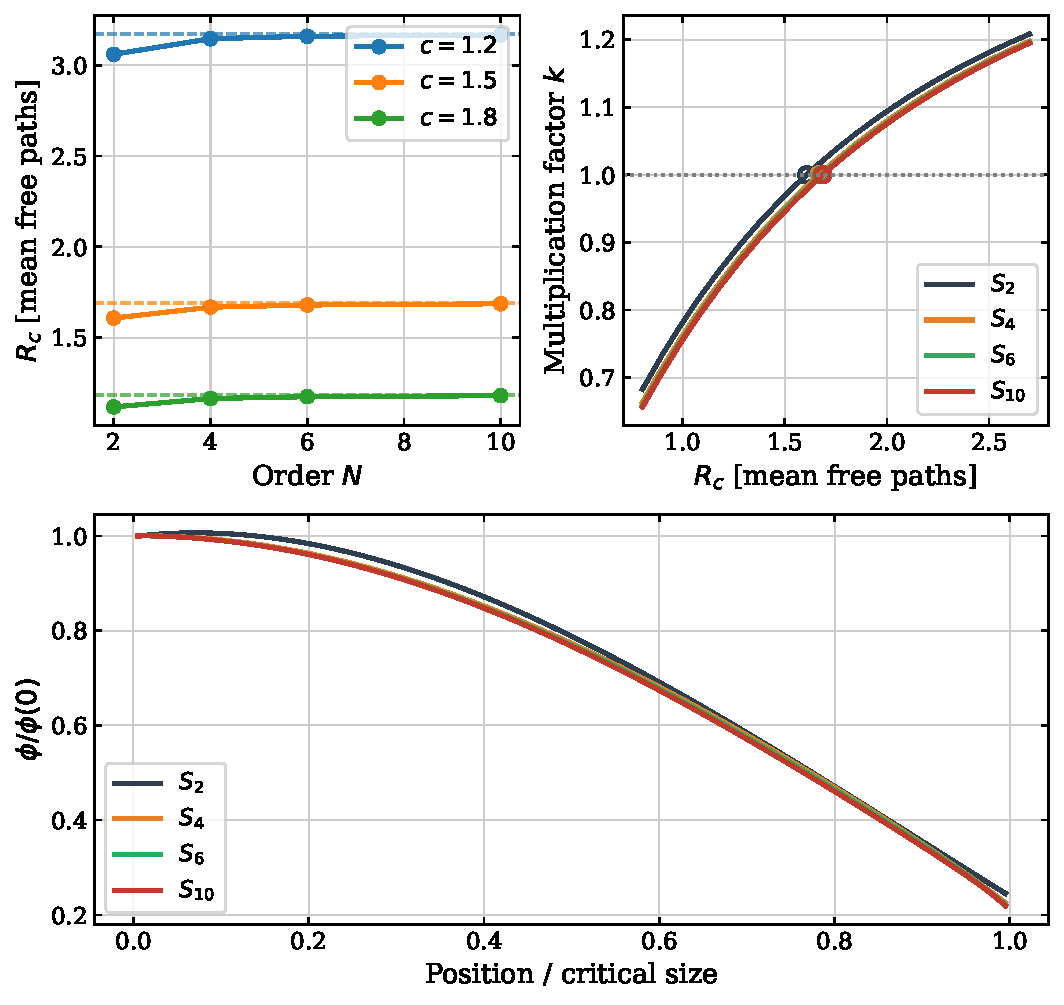
\includegraphics[width=\textwidth]{figs/q4_sphere_orders.pdf}
\caption{The same three panels for the sphere. The $S_2$ curve is the outlier in all three: in curvilinear geometry $S_2$ is not the $P_1$ equation, and the angular redistribution term it misrepresents is a loss from the interior directions.}
\end{figure}

\paragraph{Cross-check between the two geometries.} Both drive the asymptotic flux to zero at the same extrapolated surface, so $a/2 + z_0 = \tfrac{\pi}{2}\nu_0$ and $R_c + z_0 = \pi \nu_0$, and therefore
\begin{equation}
    z_0 = R_c - 2\,(a/2)
\end{equation}
which lets the two tables above check each other without any further calculation:

\begin{table}[htbp]
\centering
\begin{tabular}{cccccc}
\toprule
$c$ & from $S_2$ & from $S_4$ & from $S_6$ & from $S_{10}$ & Case's table \\
\midrule
1.2 & 0.091 & 0.509 & 0.563 & 0.583 & 0.592 \\
1.5 & 0.047 & 0.368 & 0.438 & 0.468 & 0.475 \\
1.8 & 0.032 & 0.287 & 0.354 & 0.391 & 0.397 \\
\bottomrule
\end{tabular}
\caption{Extrapolation distance $z_0$ implied by the two geometries, in mean free paths. At $S_{10}$ it is 1.5\% below Case's value at all three $c$ --- the same shortfall three times, which is the relation's own asymptotic error. At $S_2$ it nearly vanishes, which is the sharpest statement of what low-order $S_N$ gets wrong: the boundary, not the interior.}
\end{table}

\FloatBarrier
\section*{Question 5: Critical mass of U-235 and Pu-239 by $S_N$}

The cross sections are the Question 5 table of Assignment 1 --- $\Sigma_t = 0.32640$ cm$^{-1}$ for both, giving $c = 1.500$ for Pu-239 and $c = 1.300$ for U-235 --- and the critical mass follows from the converged radius as $M_c = \tfrac{4}{3}\pi R_c^3 \rho$. Here $\Sigma_s > 0$, so the inner iteration does real work: about ten sweeps per outer, against one for the $c$-only problems above. The orders are $S_2$ to $S_{16}$ rather than the $S_2$--$S_{10}$ of the previous questions, since the mass goes as the cube of the radius and is the more demanding quantity.

\begin{table}[htbp]
\centering
\begin{tabular}{ccccccc}
\toprule
material & order & $c$ & $R_c$ [cm] & $M_c$ [kg] & asympt.\ diffusion $R_c$ [cm] & departure \\
\midrule
Pu-239 & $S_2$    & 1.500 & 4.9242 & 7.852 & 5.1890 & $-5.10\%$ \\
Pu-239 & $S_4$    & 1.500 & 5.1084 & 8.767 & 5.1890 & $-1.55\%$ \\
Pu-239 & $S_8$    & 1.500 & 5.1586 & 9.028 & 5.1890 & $-0.59\%$ \\
Pu-239 & $S_{16}$ & 1.500 & 5.1730 & 9.104 & 5.1890 & $-0.31\%$ \\
\midrule
U-235 & $S_2$    & 1.300 & 7.1218 & 28.748 & 7.4339 & $-4.20\%$ \\
U-235 & $S_4$    & 1.300 & 7.3514 & 31.619 & 7.4339 & $-1.11\%$ \\
U-235 & $S_8$    & 1.300 & 7.4072 & 32.345 & 7.4339 & $-0.36\%$ \\
U-235 & $S_{16}$ & 1.300 & 7.4231 & 32.553 & 7.4339 & $-0.15\%$ \\
\bottomrule
\end{tabular}
\caption{Critical radius and mass, against the asymptotic diffusion result of Assignment 1 Question 5. The mass is the cube of the radius, so the $5\%$ radius error of $S_2$ is a $14\%$ error in mass.}
\end{table}

\begin{figure}[htbp]
\centering
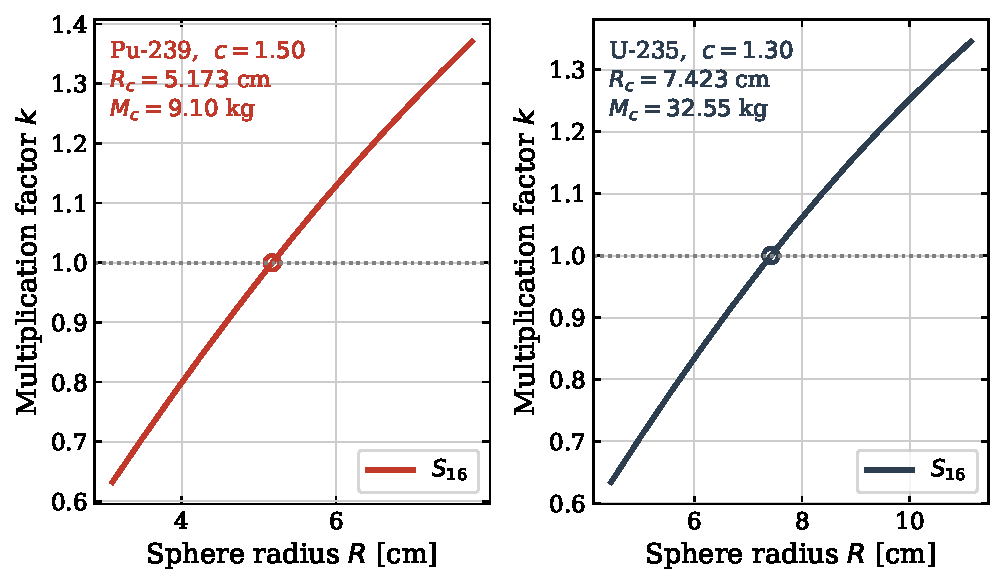
\includegraphics[width=\textwidth]{figs/q5_critical_mass.pdf}
\caption{$k$ against sphere radius at $S_{16}$, with the $k=1$ crossing that fixes the critical mass.}
\end{figure}

Diffusion overestimates both radii, and by more for Pu-239 than for U-235: the surface sits about two mean free paths from the centre in both cases, but the higher $c$ makes the Pu-239 flux fall off faster and its surface angular flux more forward-peaked, which is exactly what a diffusion approximation cannot represent. $S_{16}$ recovers the difference to within $0.3\%$ of the transport-theory radius.
\end{document}
